\documentclass{beamer}

\usetheme[secheader]{Madrid}

\usepackage{graphicx}
\graphicspath{ {./images/} }
\usepackage[table]{xcolor}


\usepackage{tikz}
\usetikzlibrary{shapes,arrows}
\usepackage[edges]{forest}
\usetikzlibrary{trees}

\usepackage{pifont}

\newcommand{\highlight}[1]{{\color{blue} #1}}
\newcommand{\pending}[1]{{\color{red} #1}}
\newcommand{\done}{{\color{green}\ding{52}}}
\newcommand{\todo}{{\color{red}\ding{56}}}
\newcommand{\doing}{{\color{orange}\ding{229}}}
\newcommand{\new}{{\colorbox{blue!30}{\textcolor{white}{\textbf{\scriptsize New!}}}}}
\newcommand{\goal}{{\colorbox{green!30}{\textcolor{white}{\textbf{\scriptsize Goal!}}}}}
\newcommand{\focus}{{\colorbox{red!30}{\textcolor{white}{\textbf{\tiny !}}}}}

\title{Tercera Reunión General del LMRI}
\subtitle{TIC: Unidad de Tecnologías de la Información y el Conocimiento}
\author[X. Campo]{Xandra Campo}
\institute[LMRI-CIEMAT]{Laboratorio de Metrología de Radiaciones Ionizantes (LMRI) \newline CIEMAT}
\date{11 de diciembre de 2024}<

\begin{document}

	\maketitle

	\begin{frame}
		\frametitle{Table of Contents}
		\tableofcontents
	\end{frame}

	\section{Unidad de TIC}
	
	\subsection{Sobre la Unidad de TIC}
	
	\begin{frame}
		\frametitle{Sobre la Unidad de TIC}
		\framesubtitle{Objetivo, cronología y organigrama}
		\begin{itemize}
			\item \highlight{Objetivo}: Proporcionar soluciones de software y/o tecnologías asociadas que respondan a las necesidades del LMRI y los laboratorios que lo componen
			\item Unidad de \highlight{nueva creación}:
			\begin{itemize}
				\item Trabajo activo desde febrero de 2024  \done
				\item Propuesta oficial en mayo de 2024 \done
				\item Clave funcional activa desde junio de 2024 \done
				\item \pending{Clave orgánica pendiente de asignación} \todo
			\end{itemize}
		\end{itemize}
%		\bigskip
		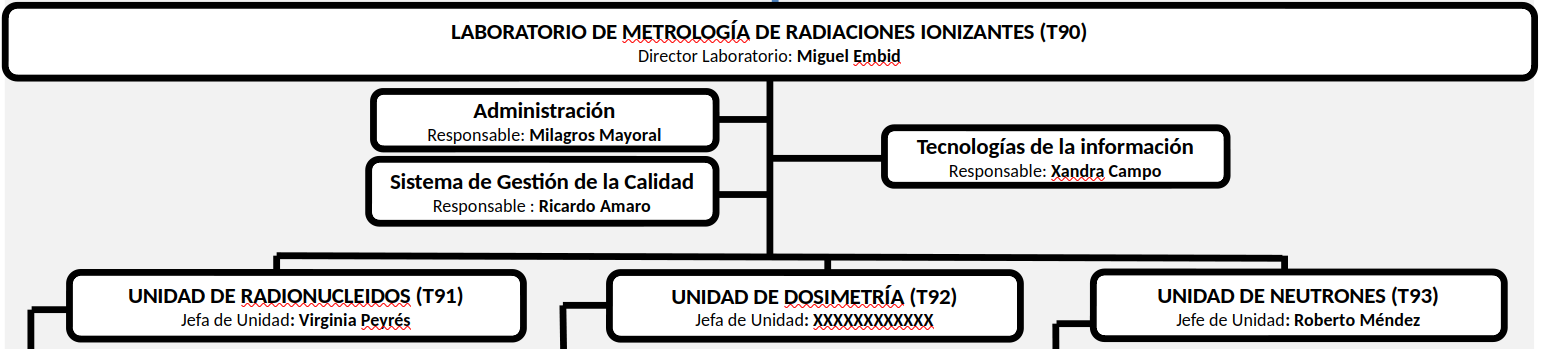
\includegraphics[width=\textwidth]{organigrama}
	\end{frame}
	
	\begin{frame}
		\frametitle{Sobre la Unidad de TIC}
		\framesubtitle{Tipos de soluciones y metodologías de trabajo}
		\centering
		\rowcolors{2}{gray!15}{white}
		\begin{tabular}{ll}
			\rowcolor{blue!40}
			{\color{white}Tipos de soluciones}&{\color{white}Herramientas de desarrollo}\\
			Librerías de Python&Librerías de Python\\
			Scripts de Python&Librerías de Python\\
			Páginas web&Flask, Django\\
			Aplicaciones web&Flask, Django\\
			Aplicaciones de escritorio&Tkinter, PyQt\\
			Formación&Seminarios, cursos, prácticas\\
			\rowcolor{blue!40}
			{\color{white}Metodologías de trabajo}&{\color{white}Herramientas de desarrollo}\\
			Entornos de trabajo&PyCharm, Git, GitHub\\
			Plataformas de difusión&GitHub, PyPI\\
		\end{tabular}
	\end{frame}

	\subsection{Proyectos}

	\begin{frame}
		\frametitle{Proyectos}
		\framesubtitle{EURAMET GuideRadPROS project}
		\begin{itemize}
			\item \highlight{Pagina web del proyecto} \done
			\begin{itemize}
				\item Prácticas estudiante FP  \done
			\end{itemize}
			\item \highlight{Librería USpekPy} \doing
			\begin{itemize}
				\item Aplicación web \doing
				\begin{itemize}
					\item Prácticas estudiante FP \done \ \goal
				\end{itemize}
				\item Seminario uso librería \done
				\item Script ficheros entrada \done
				\item Script análisis librería \done
				\item Publicar librería SpekPy \done
			\end{itemize}
			\item \highlight{Análisis de datos} \doing \ \new
			\begin{itemize}
				\item Script espectrometría experimental \done \ \new \ \goal
				\item Script medida de HVL \todo \ \new
				\item Script gráficas para análisis \todo \ \new
			\end{itemize}
		\end{itemize}
	\end{frame}

	\begin{frame}
		\frametitle{Proyectos}
		\framesubtitle{IR14-D: Patrones dosimétricos de rayos X}
		\begin{itemize}
			\item \highlight{Automatización cadena de medida} \doing
			\begin{itemize}
				\item Aplicación de escritorio calibración \doing
				\item Librería MetPyX \doing
			\end{itemize}
			\item \highlight{Aplicación lectura barómetro} \done
			\item \highlight{Scripts} \doing
			\begin{itemize}
				\item Espectrometría experimental \done \ \new \ \goal
				\item Medida de HVL \todo \ \new
				\item Calibración \doing
				\item Asignación de dosis \todo
			\end{itemize}
			\item \highlight{Librería MetPyX} \doing
		\end{itemize}
	\end{frame}

	\begin{frame}
		\frametitle{Proyectos}
		\framesubtitle{LMRI}
		\begin{itemize}
			\item \highlight{Organización GitHub} \done
			\item \highlight{Servidores LMRI} \doing
			\begin{itemize}
				\item Interno \doing
				\item Externo \doing
			\end{itemize}
			\item \highlight{Librería MetPy} \doing \ \new
			\begin{itemize}
				\item Calculo de incertidumbres \todo \ \new
				\item Interpolador \doing \ \new
			\end{itemize}
			\item \highlight{Curso ecosistema de trabajo de Python} \todo
			\item Página web LMRI
			\begin{itemize}
				\item \highlight{Modernización} de la web del LMRI \todo
				\item Aplicación web solicitud de \highlight{servicios técnicos} \doing
			\end{itemize}
		\end{itemize}
	\end{frame}
	
	\begin{frame}
		\frametitle{Proyectos}
		\framesubtitle{Herramientas públicas: enlaces de interés}
		\centering
		\scriptsize
		\rowcolors{2}{gray!15}{white}
		\begin{tabular}{ll}			
			\rowcolor{blue!40}
			{\color{white}GuideRadPROS}&\\
			Web del proyecto&https://github.com/lmri-met/sites-guideradpros\\
			&https://lmri-met.github.io/sites-guideradpros/\\
			USpekPy: Librería&https://github.com/lmri-met/uspekpy\\
			USpekPy: Seminario&https://github.com/xandratxan/uspekpy-seminar\\
			USpekPy: Análisis librería&https://github.com/xandratxan/using-uspekpy\\
			USpekPy: Generador input&https://github.com/xandratxan/uspekpy-input-generator\\
			USpekPy: Aplicación web&https://github.com/lmri-met/uspekpy-web\\
			SpekPy: Librería&https://pypi.org/project/spekpy/\\
			\rowcolor{blue!40}
			{\color{white}IR14-D}&\\
			MetPyX: Librería&https://github.com/lmri-met/metpyx\\
			\rowcolor{blue!40}
			{\color{white}LMRI}&\\
			Organización del LMRI en GitHub&https://github.com/lmri-met\\
			Librería incertidumbres&https://github.com/xandratxan/physical-magnitude\\
		\end{tabular}
	\end{frame}
	
	\subsection{Objetivos}

	\begin{frame}
		\frametitle{Objetivos}
		\framesubtitle{Segundo semestre 2024 y primer cuatrimestre 2025}
		\centering
		\scriptsize
		\rowcolors{2}{gray!15}{white}
		\begin{tabular}{lcc}
			&Segundo&Primer\\
			&semestre&cuatrimestre\\
			&2024&2025\\
			\rowcolor{blue!40}
			{\color{white}GuideRadPROS}&&\\
			USpekPy: Aplicación web&\doing&\doing\\
			USpekPy: Prácticas estudiante FP&\done&\\
			Análisis de datos: Script espectrometría experimental \focus &\done&\\
			Análisis de datos: Script medida de HVL \focus &&\todo\\
			Análisis de datos: Script gráficas para análisis \focus &&\todo\\
			\rowcolor{blue!40}
			{\color{white}IR14-D}&&\\
			Aplicación de escritorio calibración&\doing&\doing\\
			Script espectrometría experimental&\done&\\
			\rowcolor{blue!40}
			{\color{white}LMRI}&&\\
			Puesta en marcha servidor web externo&\doing&\doing\\
			Puesta en marcha servidor web interno&\doing&\textbf{?}\\
			Curso ecosistema de trabajo de Python&\todo&\textbf{?}\\
			Aplicación web solicitud de servicios técnicos*&\doing&\doing\\
		\end{tabular}
	\end{frame}
	
	\subsection{Necesidades y propuestas}
	
	\begin{frame}
		\frametitle{Necesidades y propuestas}
		\highlight{Propuestas}
		\begin{itemize}
			\item Validación de hojas de cálculo de calibración y/o asignación de dosis con scripts de Python
		\end{itemize}
		\highlight{Necesidades}
		\begin{itemize}
			\item Páginas y aplicaciones web \highlight{públicas}:
			\begin{itemize}
				\item Puesta en marcha de servidor web externo a CIEMAT
				\item Recursos propios de XCB \done
			\end{itemize}
			\item Páginas y aplicaciones web para el \highlight{LMRI}:
			\begin{itemize}
				\item Puesta en marcha de un servidor web interno
				\item Sería necesario un ordenador + monitor \doing
			\end{itemize}
		\end{itemize}
	\end{frame}
	
	\subsection{}
	
	\begin{frame}
		\begin{block}{}
			\centering
			¡Gracias por vuestra atención!
		\end{block}
	\end{frame}

\end{document}